\documentclass[10pt]{article}
\usepackage[utf8]{inputenc}
\usepackage[T1]{fontenc}
\usepackage{amsmath}
\usepackage{amsfonts}
\usepackage{amssymb}
\usepackage[version=4]{mhchem}
\usepackage{stmaryrd}
\usepackage{hyperref}
\hypersetup{colorlinks=true, linkcolor=blue, filecolor=magenta, urlcolor=cyan,}
\urlstyle{same}
\usepackage{caption}
\usepackage{graphicx}
\usepackage[export]{adjustbox}
\graphicspath{ {./images/} }

\title{Ultrafast nonlinear dynamics of surface plasmon polaritons in gold nanowires due to the intrinsic nonlinearity of metals }

\author{A Marini ${ }^{1,4}$, M Conforti ${ }^{2}$, G Della Valle ${ }^{3}$, H W Lee ${ }^{1}$, Tr X Tran ${ }^{1}$, W Chang ${ }^{1}$, M A Schmidt ${ }^{1}$, S Longhi ${ }^{3}$, P St J Russell ${ }^{1}$ and F Biancalana ${ }^{1,4}$\\
${ }^{1}$ Max Planck Institute for the Science of Light, Guenther-Scharowsky-Straße 1, D-91058 Erlangen, Germany\\
${ }^{2}$ CNISM and Dipartimento di Ingegneria dell’Informazione, Universitá degli Studi di Brescia, Via Branze 38, I-25123 Brescia, Italy\\
${ }^{3}$ Dipartimento di Fisica, Politecnico di Milano, and IFN-CNR, Piazza Leonardo da Vinci 32, I-20133 Milano, Italy\\
E-mail: Andrea.Marini@mpl.mpg.de and Fabio.Biancalana@mpl.mpg.de}
\date{}


%New command to display footnote whose markers will always be hidden
\let\svthefootnote\thefootnote
\newcommand\blfootnotetext[1]{%
  \let\thefootnote\relax\footnote{#1}%
  \addtocounter{footnote}{-1}%
  \let\thefootnote\svthefootnote%
}

%Overriding the \footnotetext command to hide the marker if its value is `0`
\let\svfootnotetext\footnotetext
\renewcommand\footnotetext[2][?]{%
  \if\relax#1\relax%
    \ifnum\value{footnote}=0\blfootnotetext{#2}\else\svfootnotetext{#2}\fi%
  \else%
    \if?#1\ifnum\value{footnote}=0\blfootnotetext{#2}\else\svfootnotetext{#2}\fi%
    \else\svfootnotetext[#1]{#2}\fi%
  \fi
}

\begin{document}
\maketitle
\captionsetup{singlelinecheck=false}
\section*{PAPER•OPEN ACCESS}
\section*{Ultrafast nonlinear dynamics of surface plasmon polaritons in gold nanowires due to the intrinsic nonlinearity of metals}
To cite this article: A Marini et al 2013 New J. Phys. 15013033

View the article online for updates and enhancements.

\section*{You may also like}
\begin{itemize}
  \item Electron enerqy can oscillate near a crystal dislocation Mingda Li, Wenping Cui, Mildred S Dresselhaus et al.
  \item Tailoring near-field-mediated photon electron interactions with light polarization Fatemeh Chahshouri and Nahid Talebi
  \item Comparing complex networks: in defence of the simple\\
Johann H Martínez and Mario Chavez
\end{itemize}

New Journal of Physics 15 (2013) 013033 (19pp)\\
Received 7 August 2012\\
Published 16 January 2013\\
Online at \href{http://www.njp.org/}{http://www.njp.org/}\\
doi:10.1088/1367-2630/15/1/013033

\begin{abstract}
Starting from first principles, we theoretically model the nonlinear temporal dynamics of gold-based plasmonic devices resulting from the heating of their metallic components. At optical frequencies, the gold susceptibility is determined by the interband transitions around the $X, L$ points in the first Brillouin zone, and thermo-modulational effects ensue from Fermi smearing of the electronic energy distribution in the conduction band. As a consequence of light-induced heating of the conduction electrons, the optical susceptibility becomes nonlinear. In this paper we describe, for the first time to our knowledge, the effects of the thermo-modulational nonlinearity of gold on the propagation of surface plasmon polaritons guided on gold nanowires. We introduce a novel nonlinear Schrödinger-like equation to describe pulse propagation in such nanowires, and we predict the appearance of an intense spectral red-shift caused by the delayed thermal response.
\end{abstract}

\footnotetext{${ }^{4}$ Authors to whom any correspondence should be addressed.
}\section*{Contents}
\begin{enumerate}
  \item Introduction and motivations ..... 2
  \item Optical properties of gold ..... 4
  \item Electron temporal dynamics and the two-temperature model ..... 6
  \item Thermo-modulational interband nonlinear susceptibility ..... 8
  \item Thermo-modulational nonlinear dynamics in plasmonic devices ..... 10\\
5.1. Linear modes ..... 10\\
5.2. The generalized nonlinear Schrödinger equation ..... 13
  \item Summary ..... 17\\
Acknowledgments ..... 18\\
References ..... 18
\end{enumerate}

\section*{1. Introduction and motivations}
The design and development of subwavelength photonic devices with metallic components has become a subject of intense research over the last decade. This trend is justified by the need for compact high-performance optical devices and is mainly driven by the enormous technological improvement in nano-fabrication techniques. These state-of-the-art manufacturing tools for metallic nano-circuits have made it possible to design and engineer the effective optical properties of artificial materials, commonly known as metamaterials. In these synthetic materials, the propagation of light is strongly influenced by the geometric properties of the embedded metallic nano-circuits. In particular, the metallic nano-structures can be tailored in such a way that the effective refractive index becomes negative [1]. Negative index materials are potentially important in superlensing [2] and cloaking applications [3]. Novel physical mechanisms occur in anisotropic metamaterials, which under some circumstances can exhibit hyperbolic dispersion [4]. In the nonlinear regime, metamaterials have been studied for harmonic generation [5], soliton propagation [6] and optical modulation and switching [7]. The unusual properties of metamaterials arise from the fact that the metallic nano-circuits are much smaller than the wavelength of light, resulting in a space-averaged macroscopic dielectric response. Conversely, in the case where the optical wavelength is comparable with the dimensions of the metallic sub-structures, the light feels the geometric details and plasmon polariton modes are excited. Surface plasmon polaritons (SPPs) are electromagnetic waves propagating on metallic surfaces. They constitute the best candidates for manipulating light on the nanoscale and for the development of subwavelength all-optical devices [8]. In particular, plasmonic waveguides have important applications as optical interconnects in highly integrated optoelectronic devices [9]. Other relevant applications of SPPs are found in medicine [10], sensing [11] and nano-lasers [12]. The nonlinear properties of SPPs can be used for second harmonic generation [13], active control [14] and nanofocusing [15]. Nonlinear self-action can be exploited for manipulating transverse spatial diffraction by selffocusing and for the formation of plasmon solitons [16, 17]. Subwavelength modulational instability, plasmon oscillon formation and nonlinear switching can be achieved in arrays of\\[0pt]
metallic nanoparticles [18, 19]. Fundamental studies of metamaterials and SPPs are closely related. Indeed, relevant phenomena occurring in metamaterials are observed also in plasmonics, e.g. negative refraction [20], anomalous diffraction [21, 22] and electromagnetic cloaking [23]. In both fields, an innovative step is the use of nanostructured metals for manipulating light. In most of the nonlinear studies reported above, the optical response of metals is assumed to be linear, while the nonlinearity originates from the dielectric medium; however, experimentalists know well that the Kerr nonlinearity of metals can be enormous. Experimental results indicate strong third-order nonlinear susceptibilities that vary by several orders of magnitude, with values of $\chi_{3}^{m}$ that vary between $10^{-14}$ and $10^{-18} \mathrm{~m}^{2} \mathrm{~V}^{-2}[24,25]$ and that are much bigger than the third-order susceptibility of bulk silica $\left(\chi_{3}^{\mathrm{Si}} \approx 10^{-22} \mathrm{~m}^{2} \mathrm{~V}^{-2}\right)$. Recently, the non-local ponderomotive nonlinearity for a plasma of free electrons was proposed as a possible model for the interpretation of experimental results [26]. The predicted value for the ponderomotive third-order susceptibility at optical frequencies ( $\chi_{3} \approx 10^{-20} \mathrm{~m}^{2} \mathrm{~V}^{-2}$ ) is, however, insufficient to explain the experimental findings. In addition, the spectral dependence of the ponderomotive nonlinearity ( $\chi_{3} \propto 1 / \omega^{4}$ ) does not fit with the enormous spectral variation (by several orders of magnitude) observed in the measurements, suggesting that the basic nonlinear mechanism for metals is resonant. Theoretical and experimental confirmation of this hypothesis is to be found in the results of Rosei, Guerrisi et al on the thermo-modulational reflection spectra of thin films of noble metals [27,28]. In their work, the authors theoretically predict and experimentally observe a strong modulation in the reflection spectrum due to light-induced heating. They demonstrate that the temperature change smears out the energy distribution of the conduction electrons, affecting the resonant interband absorption and hence the dielectric susceptibility. This process is intrinsically nonlinear, since the temperature change modulating the dielectric response depends on the optical power. Subsequent pump-probe experiments in thin films [29] and nanoparticles [30] have confirmed the initial results of Rosei and Guerrisi. Theoretical and experimental investigations on the temporal dynamics of the system clearly indicate that the nonlinear response of metals is characterized by a delayed mechanism [31], as is typical of thermal nonlinearities. Very recently, a complete analysis of the nonlinear optical response of noble metals, leading to the first theoretical derivation of a consistent model for the third-order nonlinear susceptibility of gold, was reported [32]. Although experiments in thin films have been satisfactorily explained, a theoretical description of the thermo-modulational interband nonlinearity for ultrashort optical pulses propagating in plasmonic waveguides is still missing.

In this paper, we describe the effects of the thermo-modulational nonlinear susceptibility on SPPs propagating in a gold nanowire surrounded by silica glass. The paper is organized as follows. In section 2 we briefly describe the optical properties of gold, the interband transitions, their effect on the dielectric susceptibility and its temperature dependence. Then, in section 3, we model the temporal dynamics of the electrons through the two-temperature model (TTM), deriving the characteristic temporal response function. In section 4, collecting the results of the previous sections, we are able to derive an analytical expression for the thermo-modulation interband polarization. Finally, in section 5, we model the propagation of SPPs along a gold nanowire by introducing a novel nonlinear Schrödinger-like equation and predicting for the first time to our knowledge a strong red-shift caused by the thermo-modulational nonlinearity of gold.

\section*{2. Optical properties of gold}
The non-resonant optical properties of gold can be described through the free-electron model, where electrons are considered to be free charges moving in response to an optical field $\operatorname{Re}\left[\vec{E}_{0} \mathrm{e}^{-\mathrm{i} \omega t}\right]$ oscillating at angular frequency $\omega$. In this model, the dielectric response of the plasma can be derived directly from the non-relativistic single-particle equation of motion: $\epsilon_{\text {intra }}(\omega)=1-\omega_{\mathrm{p}}^{2} /\left(\omega^{2}+\mathrm{i} \gamma \omega\right)$, where $\omega_{\mathrm{p}}=\sqrt{n e^{2} / \epsilon_{0} m_{\mathrm{e}}}$ is the plasma frequency, $\epsilon_{0}$ is the vacuum permittivity, $n$ is the electron number density, $e, m_{\mathrm{e}}$ are the electron charge and mass and $\gamma$ is a characteristic frequency accounting for electron-electron collisions. This model is justified by the fact that for metals the Fermi energy lies within the conduction band and many accessible states exist for the electrons. From a quantum perspective, free-electron motion only accounts for intraband transitions. For wavelengths in the far infrared, the free-electron model provides very good quantitative agreement with experimental data [33]. For the free-electron calculations we use the parameters $\omega_{\mathrm{p}}=1.1515 \times 10^{16} \mathrm{rad} \mathrm{s}^{-1}, \gamma=8.9890 \times 10^{13} \mathrm{~s}^{-1}$, obtained by fitting $\epsilon_{\text {intra }}^{\prime \prime}(\omega)$ to the experimental data for long wavelengths in the far infrared. At optical frequencies and in the near infrared, the susceptibility of gold is more involved and the non-resonant model is not sufficient to explain the experimental measurements. Indeed, interband transitions between the $d$-band and the conduction band become important and cannot be neglected. The presence of interband transitions enriches the variety of physical processes and lies behind the strong temperature dependence of the dielectric susceptibility. At optical frequencies, the gold dielectric susceptibility measured in experiments [33] deviates significantly from the predictions of the free-electron model as a consequence of two intense interband absorption peaks at $\lambda=300$ and 410 nm . Thus, the actual dielectric constant of gold can be expressed as the sum $\epsilon_{m}(\omega)=\epsilon_{\text {intra }}(\omega)+\epsilon_{\text {inter }}(\omega)$.

Gold is characterized by a face centered cubic lattice structure, where the Wigner-Seitz primitive cell is a rhombic dodecahedron. The reciprocal lattice is a body centered cubic where the Wigner-Seitz primitive cell is a truncated octahedron. At optical frequencies, the interband absorption is resonant around the points $X$ and $L$ in reciprocal space [28], which correspond, respectively, to the centers of the square and hexagonal facets of the truncated octahedron. Notably, such points are highly symmetric and around them the lattice vector $\vec{k}$ can be expressed as the sum $\vec{k}=\vec{k}_{\perp}+\vec{k}_{\|}$, where $\vec{k}_{\perp}$ lies on the square ( $X$ ) or hexagonal ( $L$ ) facets and $\vec{k}_{\|}$is perpendicular to them. In addition, the Fermi surface has cylindrical symmetry around the $X, L$ points and the valence and conduction bands can be approximated in ( $k_{\perp}, k_{\|}$) space by elliptic and hyperbolic paraboloids [28]:


\begin{equation*}
E_{\mathrm{v}}(\vec{k})=E_{0 \mathrm{v}}-\frac{\hbar^{2} k_{\perp}^{2}}{2 m_{\mathrm{v} \perp}}-\frac{\hbar^{2} k_{\|}^{2}}{2 m_{\mathrm{v} \|}}, \quad E_{\mathrm{c}}(\vec{k})=E_{0 \mathrm{c}}+\frac{\hbar^{2} k_{\perp}^{2}}{2 m_{\mathrm{c} \perp}}-\frac{\hbar^{2} k_{\|}^{2}}{2 m_{\mathrm{c} \|}}, \tag{1}
\end{equation*}


where $\mathrm{v}, \mathrm{c}$ indicate the valence and conduction bands. The values of the constants $E_{0 \mathrm{v}}, E_{0 \mathrm{c}}$, $m_{\mathrm{v} \perp}, m_{\mathrm{c} \perp}, m_{\mathrm{v} \|}, m_{\mathrm{c} \|}$ for the $X$ and $L$ transitions that we use in our calculations are known in the literature [28]. Note that, as a consequence of the cylindrical symmetry of the Fermi surface, the conduction and valence bands around the $X, L$ points do not depend on the direction of $\vec{k}_{\perp}$, but only on its modulus $k_{\perp}$. The Fermi level $E_{\mathrm{F}}$ lies in the conduction band $E_{\mathrm{c}}(\vec{k})$ and for the sake of simplicity (and without loss of generality) we perform a constant shift of all energies and assume that $E_{\mathrm{F}}=0$. Note that the paraboloid approximation made in (1) is accurate only if $k_{\perp}, k_{\|} \ll k_{\Gamma}$, where $k_{\Gamma}$ is the distance between the $X, L$ points and the center of the Brillouin zone. The quantum states of electrons in the valence and conduction bands are Bloch\\
wavefunctions $\psi_{\mathrm{v}, \mathrm{c}}=\Omega^{-1 / 2} u_{\vec{k}, \mathrm{v}, \mathrm{c}}(\vec{r}) \exp (\mathrm{i} \vec{k} \cdot \vec{r})$, where $\Omega$ is the primitive cell volume, $\vec{k}$ is the Brillouin wavevector and $u_{\vec{k}, \mathrm{v}, \mathrm{c}}(\vec{r})$ are the unit cell wavefunctions. By using the Fermi golden rule and following the procedure reported in [27,28,32], it is possible to calculate the imaginary part of the dielectric constant due to the $X, L$ interband transitions


\begin{equation*}
\epsilon_{\text {inter }}^{\prime \prime}\left(\omega, T_{\mathrm{e}}\right)=\frac{\pi e^{2}}{3 \epsilon_{0} m_{\mathrm{e}}^{2} \omega^{2}}\left[\left|\vec{p}_{\mathrm{c}, \mathrm{v}}^{X}\right|^{2} J_{\mathrm{c}, \mathrm{v}}^{X}\left(\omega, T_{\mathrm{e}}\right)+\left|\vec{p}_{\mathrm{c}, \mathrm{v}}^{L}\right|^{2} J_{\mathrm{c}, \mathrm{v}}^{L}\left(\omega, T_{\mathrm{e}}\right)\right] \tag{2}
\end{equation*}


where $\vec{p}_{\mathrm{v}, \mathrm{c}}=-\mathrm{i}(\hbar / \Omega) \int_{\Omega} \mathrm{d}^{3} r\left[u_{\vec{k}, \mathrm{v}}^{*}(\vec{r}) \nabla u_{\vec{k}, \mathrm{c}}(\vec{r})\right]$ is the dipole matrix element and $J_{\mathrm{c}, \mathrm{v}}\left(\omega, T_{\mathrm{e}}\right)$ is the joint density of states (JDOS)


\begin{equation*}
J_{\mathrm{c}, \mathrm{v}}\left(\omega, T_{\mathrm{e}}\right)=\frac{2}{(2 \pi)^{3}} \int_{\mathrm{BZ}} \mathrm{~d}^{3} k\left\{\delta\left[E_{\mathrm{c}}(\vec{k})-E_{\mathrm{v}}(\vec{k})-\hbar \omega\right] f\left[E_{\mathrm{v}}(\vec{k}), T_{\mathrm{e}}\right]\left(1-f\left[E_{\mathrm{c}}(\vec{k}), T_{\mathrm{e}}\right]\right)\right\} \tag{3}
\end{equation*}


In the equation above, $T_{\mathrm{e}}$ is the electronic temperature and $f\left(E, T_{\mathrm{e}}\right)$ is the Fermi-Dirac occupation number. Note that the conservation of energy and the Pauli exclusion principle for every $\mathrm{v} \rightarrow \mathrm{c}$ direct transition are carefully considered in the expression for $J_{\mathrm{c}, \mathrm{v}}$. Indeed, the factor $f\left[E_{\mathrm{v}}(\vec{k}), T_{\mathrm{e}}\right]$ accounts for the probability that the $\vec{k}$-state in the valence band is occupied, while the factor $1-f\left[E_{\mathrm{c}}(\vec{k}), T_{\mathrm{e}}\right]$ accounts for the probability that the $\vec{k}$-state in the conduction band is empty. The real part of the dielectric constant can then be obtained directly from (2) using the Kramers-Kronig relation


\begin{equation*}
\epsilon_{\text {inter }}^{\prime}\left(\omega, T_{\mathrm{e}}\right)=\frac{1}{\pi} \mathcal{P} \int_{-\infty}^{+\infty} \frac{\epsilon_{\text {inter }}^{\prime \prime}\left(\omega^{\prime}, T_{\mathrm{e}}\right)}{\omega^{\prime}-\omega} \mathrm{d} \omega^{\prime} \tag{4}
\end{equation*}


where $\mathcal{P}$ represents the principal value of the integral. If the conduction electrons are taken out of equilibrium by light-induced heating, the interband absorption is affected by the so-called Fermi smearing effect [28]. Increasing temperature broadens the electron distribution around the Fermi energy, modifying the effective optical properties of gold. In order to understand the temperature dependence of $\epsilon_{\text {inter }}^{\prime \prime}$, contained in the $X, L$ JDOSs, one needs to compute numerically the thermo-derivatives $\partial_{T_{\mathrm{e}}} J_{\mathrm{c}, \mathrm{V}}^{X, L}\left(\omega, T_{\mathrm{e}}\right)$. For the dipole matrix elements $\left|\vec{p}_{\mathrm{c}, \mathrm{V}}^{X}\right|^{2},\left|\vec{p}_{\mathrm{c}, \mathrm{V}}^{L}\right|^{2}$ we have used the values $g_{L}\left|\vec{p}_{\mathrm{c}, \mathrm{v}}^{L}\right|^{2}=1.6015 \times 10^{-47} \mathrm{~J} \mathrm{~kg}, g_{X}\left|\vec{p}_{\mathrm{c}, \mathrm{V}}^{X}\right|^{2}=0.321 \times g_{L}\left|\vec{p}_{\mathrm{c}, \mathrm{V}}^{L}\right|^{2}$, where $g_{L}=8, g_{X}=6[28,34]$. The resulting interband dielectric thermo-derivative can be fitted to a series of five Lorentzian functions:


\begin{equation*}
\partial_{T_{\mathrm{e}}} \epsilon_{\text {inter }}^{\prime \prime}(\omega)=\sum_{j=1}^{5} \frac{\mathcal{F}_{j} \omega_{\mathrm{p}}^{2}}{\left(\omega-\omega_{j}\right)^{2}+\gamma_{j}^{2}}, \tag{5}
\end{equation*}


where $\omega_{\mathrm{p}}$ is the plasma frequency of gold. The fit parameters are given in table 1. The calculation of the real part $\partial_{T_{\mathrm{e}}} \epsilon_{\text {inter }}^{\prime}$ through the integration of the Kramers-Kronig relation given by (4) is straightforward:


\begin{equation*}
\partial_{T_{\mathrm{e}}} \epsilon_{\text {inter }}^{\prime}(\omega)=\sum_{j=1}^{5} \frac{\mathcal{F}_{j} \omega_{\mathrm{p}}^{2}\left(\omega_{j}-\omega\right)}{\gamma_{j}\left(\omega-\omega_{j}\right)^{2}+\gamma_{j}^{3}} . \tag{6}
\end{equation*}


As light impinges on the gold surface, the electrons in the conduction band are heated and the dielectric constant is modified by the amount $\Delta \epsilon_{m}(\omega)=\partial_{T_{\mathrm{e}}} \epsilon_{\text {inter }}(\omega) \Delta T_{\mathrm{e}}$.

Note that this thermo-modulational process is intrinsically nonlinear, since the increase of temperature depends on the absorbed optical power $\Delta T_{\mathrm{e}}\left(P_{\mathrm{A}}\right)$. The spectral dependence of the

\begin{table}[h]
\begin{center}
\captionsetup{labelformat=empty}
\caption{Table 1. Fit parameters for the thermo-derivative $\partial_{T_{\mathrm{e}}} \epsilon_{\mathrm{inter}}^{\prime \prime}(\omega)$, given by (5). $\omega_{\mathrm{p}}= 1.1515 \times 10^{16} \mathrm{rad} \mathrm{s}^{-1}$ is the plasma frequency of gold, which has been calculated by fitting the experimental data in the far infrared with the free-electron model.}
\begin{tabular}{lrrrrr}
\hline
$j$ & 1 & 2 & 3 & 4 & 5 \\
\hline
$\mathcal{F}_{j} \times 10^{7}$ & -1.6969 & -2.9413 & +5.0681 & -1.0016 & +0.4045 \\
$\omega_{j} / \omega_{\mathrm{p}}$ & 0.3982 & 0.3541 & 0.3140 & 0.2587 & 0.2238 \\
$\gamma_{j} / \omega_{\mathrm{p}}$ & 0.0217 & 0.0216 & 0.0173 & 0.0217 & 0.0130 \\
\hline
\end{tabular}
\end{center}
\end{table}

\begin{figure}[h]
\begin{center}
  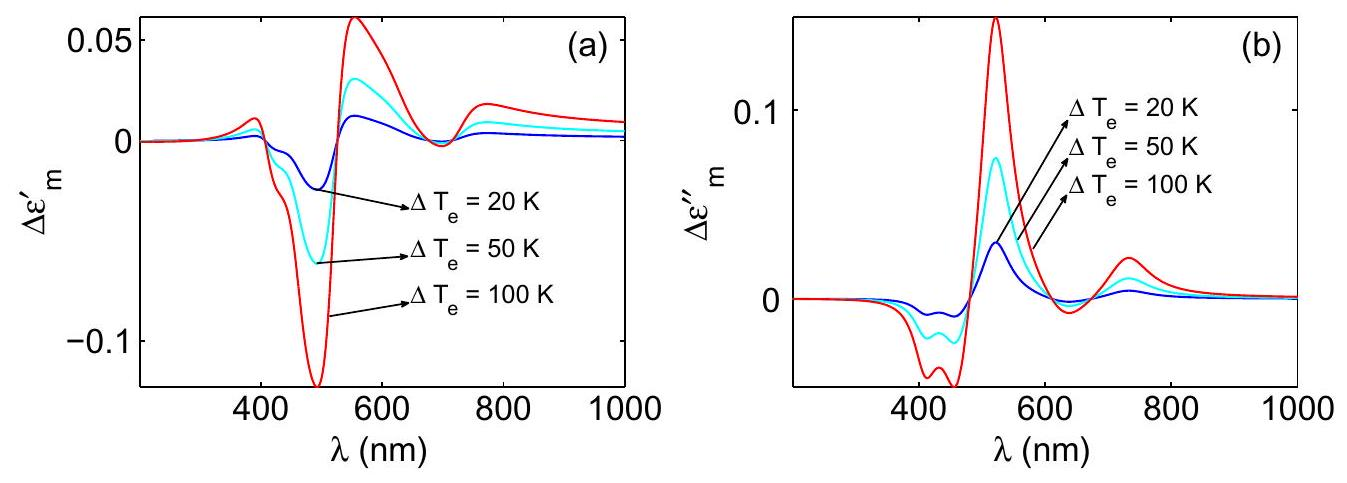
\includegraphics[alt={},max width=\textwidth]{fedff7ea-fb9d-4a80-ac6f-348dbc7a5487-07_483_1347_868_497}
\captionsetup{labelformat=empty}
\caption{Figure 1. Thermo-modulation of the dielectric constant of gold. (a) Real and (b) imaginary corrections to the dielectric constant $\Delta \epsilon_{m}=\partial_{T_{\mathrm{e}}} \epsilon_{\text {inter }}\left(\omega, T_{0}\right)\left(T_{\mathrm{e}}-\right. \left.T_{0}\right)\left(T_{0}=300 \mathrm{~K}\right)$. Blue, cyan and red curves correspond to the electronic temperatures $T_{\mathrm{e}}=320,350$ and 400 K , respectively.}
\end{center}
\end{figure}

complex correction $\Delta \epsilon_{m}(\omega)$ is plotted in figures 1(a) and (b) for several values of temperature variation $\Delta T_{\mathrm{e}}=20,50,100 \mathrm{~K}$ (blue, cyan and red curves, respectively). Note that the spectral dependence of both the real and imaginary parts $\Delta \epsilon_{m}^{\prime}(\omega), \Delta \epsilon_{m}^{\prime \prime}(\omega)$ is non-trivial and they can be either positive or negative; hence the optical absorption can increase or decrease, depending on the wavelength $\lambda$.

\section*{3. Electron temporal dynamics and the two-temperature model}
An optical beam impinging on a metal surface modifies the effective interband susceptibility by heating the electrons in the conduction band. This light-induced electron heating can be described through the TTM, which takes into account the energy balance between the conduction electrons and the lattice. The electrons have a relatively small heat capacity and so thermalize through electron-electron collisions with a characteristic time of order $\tau_{\text {th }} \approx 300 \mathrm{fs}$. If one wishes to describe the temporal electron dynamics for ultrashort optical pulses ( $\tau_{0} \approx$ 100 fs ), it is necessary to include also the energy contribution of the non-thermalized electrons in the energy balance. This can be calculated directly from the Boltzmann equation in the relaxation time approximation [31]. A phenomenological description of the electron temporal dynamics can be obtained by separating the electron distribution of energy into thermalized and\\
non-thermalized parts:


\begin{align*}
& \partial_{t} N(t)=-\left(\gamma_{\mathrm{e}}+\gamma_{1}\right) N(t)+P_{\mathrm{A}}(t) \\
& C_{\mathrm{e}} \partial_{t} T_{\mathrm{e}}(t)=\mathcal{C}\left(T_{1}-T_{\mathrm{e}}\right)+\gamma_{\mathrm{e}} N(t)  \tag{7}\\
& C_{1} \partial_{t} T_{1}(t)=\mathcal{C}\left(T_{\mathrm{e}}-T_{1}\right)+\gamma_{1} N(t)
\end{align*}


where $P_{\mathrm{A}}(t)$ is the mean absorbed power per unit volume, $T_{\mathrm{e}}(t), T_{1}(t)$ are the electronic and lattice temperatures, $C_{\mathrm{e}}, C_{1}$ are the electronic and lattice heat capacities per unit volume and $N(t)$ is the energy density stored in the non-thermalized part of the electronic distribution. When an ultrashort optical pulse impinges on the metal, it is absorbed and transfers energy to the non-thermalized electrons. In turn, the non-thermalized electrons release energy density $\gamma_{\mathrm{e}} N(t)$ to the thermalized electrons via electron-electron scattering and energy density $\gamma_{1} N(t)$ to the lattice via electron-phonon scattering. The non-thermalized electrons achieve thermal equilibrium with a characteristic time delay of $\tau_{\mathrm{th}}=\left(\gamma_{\mathrm{e}}+\gamma_{1}\right)^{-1}$, where $\gamma_{\mathrm{e}}, \gamma_{1}$ are the electron and lattice thermalization rates. Once heated by an ultrashort optical pulse, the thermalized electrons gradually release energy to the lattice via electron-phonon scattering, which is accounted for by the coupling coefficient $\mathcal{C}$. Ultimately, for long times, the electrons reach thermal equilibrium with the lattice. The parameters used in the numerical calculation are known in the literature [29]. Note that since the lattice heat capacity is much larger than the electron heat capacity, while the temporal variation of the electronic temperature $T_{\mathrm{e}}(t)$ is significant, the lattice temperature $T_{1}(t)$ does not change significantly with time, i.e. $T_{1}(t) \approx$ const. Note also that the electronic and lattice heat capacities $C_{\mathrm{e}}, C_{\mathrm{l}}$, in principle, depend on their respective temperatures $T_{\mathrm{e}}, T_{1}$ so that the extended TTM model is nonlinear. However, in the limit $\Delta T_{\mathrm{e}}(t) \ll T_{\text {eq }}$, it is possible to approximate $C_{\mathrm{e}}, C_{1}$ as independent of their respective temperatures [31]. Setting $\partial_{t} N=0$ and removing the equation for $N(t)$ is equivalent to neglecting the thermalization time $\tau_{\text {th }} \approx 300$ fs over which non-thermalized electrons release energy to the thermalized ones. For pulses of duration $\tau_{0} \approx 100$ fs such an approximation is not feasible and all the equations must be retained in order to describe correctly the delayed nonlinearity. The TTM model can be solved straightforwardly in the Fourier domain, leading to the solution


\begin{equation*}
\Delta T_{\mathrm{e}}(\Delta \omega)=T_{\mathrm{e}}(\Delta \omega)-T_{1}(\Delta \omega)=\tau_{\mathrm{r}} \tau_{\mathrm{th}}\left(\frac{\gamma_{\mathrm{e}}}{C_{\mathrm{e}}}-\frac{\gamma_{1}}{C_{\mathrm{l}}}\right) h_{\mathrm{T}}(\Delta \omega) P_{\mathrm{A}}(\Delta \omega) \tag{8}
\end{equation*}


where $\Delta \omega$ is the shift from the carrier angular frequency $\omega_{0}$ of the ultrashort optical pulse and $h_{\mathrm{T}}(\Delta \omega)=\left[1-\mathrm{i} \tau_{\mathrm{th}} \Delta \omega\right]^{-1}\left[1-\mathrm{i} \tau_{\mathrm{r}} \Delta \omega\right]^{-1}$. In the expressions above we have used the parameter $\tau_{\mathrm{r}}=C_{\mathrm{e}} C_{1} /\left[\mathcal{C}\left(C_{\mathrm{e}}+C_{1}\right)\right]$ representing the relaxation time of the thermalized electrons with the lattice. In the temporal domain, the temperature variation $\Delta T_{\mathrm{e}}(t)=T_{\mathrm{e}}(t)-T_{1}(t)$ is given by


\begin{equation*}
\Delta T_{\mathrm{e}}(t)=\tau_{\mathrm{r}} \tau_{\mathrm{th}}\left(\frac{\gamma_{\mathrm{e}}}{C_{\mathrm{e}}}-\frac{\gamma_{1}}{C_{\mathrm{l}}}\right) \int_{-\infty}^{+\infty} h_{\mathrm{T}}\left(t^{\prime}\right) P_{\mathrm{A}}\left(t-t^{\prime}\right) \mathrm{d} t^{\prime} \tag{9}
\end{equation*}


where $h_{\mathrm{T}}(t)=\theta(t)\left(\tau_{\mathrm{th}}-\tau_{\mathrm{r}}\right)^{-1}\left(\mathrm{e}^{-t / \tau_{\mathrm{th}}}-\mathrm{e}^{-t / \tau_{\mathrm{r}}}\right)$ is the temporal response function. Note that causality is imposed by means of the Heaviside step function $\theta(t)$. Note also that in the limit $P_{\mathrm{A}} \rightarrow 0$ the conduction electrons and the lattice are in equilibrium and have the same temperature $T_{\mathrm{e}}=T_{1}=T_{\mathrm{eq}}$. Since the heat capacity of the lattice $C_{1}$ is much greater than the electronic heat capacity $C_{\mathrm{e}}$, the temperature difference $\Delta T_{\mathrm{e}}(t)=T_{\mathrm{e}}(t)-T_{1}(t)$ can be approximated by $\Delta T_{\mathrm{e}}(t) \approx T_{\mathrm{e}}(t)-T_{\text {eq }}$. The response functions in the frequency $h_{\mathrm{T}}(\Delta \omega)$ and temporal $h_{\mathrm{T}}(t)$ domains are plotted as functions of $\Delta \omega$ and $t$ in figures 2(a) and (b).

\begin{figure}[h]
\begin{center}
  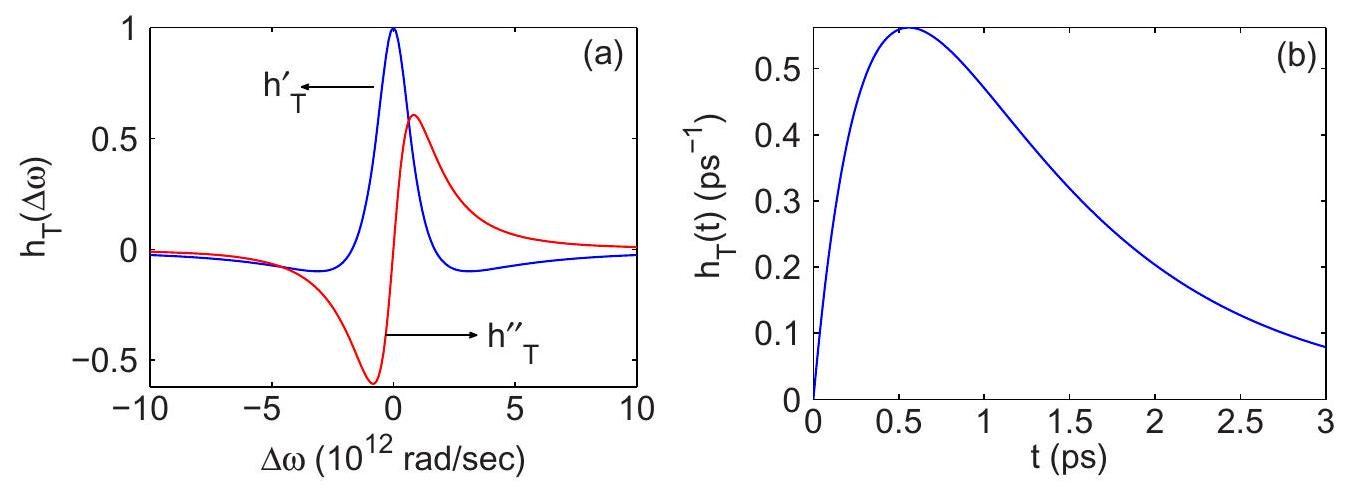
\includegraphics[alt={},max width=\textwidth]{fedff7ea-fb9d-4a80-ac6f-348dbc7a5487-09_490_1354_367_497}
\captionsetup{labelformat=empty}
\caption{Figure 2. Plot of the TTM response. (a) Fourier transform $h_{\mathrm{T}}(\Delta \omega)$ as a function of angular frequency shift $\Delta \omega$. The blue and red curves represent the real $\left(h_{\mathrm{T}}^{\prime}(\Delta \omega)\right)$ and imaginary ( $h_{\mathrm{T}}^{\prime \prime}(\Delta \omega)$ ) parts. (b) TTM temporal response $h_{\mathrm{T}}(t)$ as a function of time $t$.}
\end{center}
\end{figure}

In figure 2(a), the blue and red curves correspond to the real $h_{\mathrm{T}}^{\prime}(\Delta \omega)$ and imaginary $h_{\mathrm{T}}^{\prime \prime}(\Delta \omega)$ parts. Note that, following the sign convention chosen for the exponential in the Fourier expansion ( $\mathrm{e}^{-\mathrm{i} \Delta \omega t}$ ), a positive value of the imaginary part $h_{\mathrm{T}}^{\prime \prime}(\Delta \omega)$ corresponds to loss, while a negative value corresponds to gain. The temporal thermal response $h_{\mathrm{T}}(t)$, depicted in figure 2(b), is mainly characterized by a peak delayed in time by $\Delta t \approx 600 \mathrm{fs}$. As a consequence of the delay, blue-shifted frequency components are suppressed, while red-shifted components are amplified, analogously to what happens in solid-core optical fibers as a result of the Raman effect.

\section*{4. Thermo-modulational interband nonlinear susceptibility}
In this paragraph we sum up the results obtained so far calculating the nonlinear susceptibility due to Fermi smearing of the conduction electrons. The instantaneous power per unit volume absorbed by a metal is $W(t)=\vec{E}(t) \cdot \partial_{t} \vec{D}(t)$, where $\vec{D}(t)$ is the displacement vector. In the continuous wave (CW) monochromatic case, the electric and displacement fields are $\vec{E}(t)=\vec{E}_{0} \mathrm{e}^{-\mathrm{i} \omega_{0} t}$ and $\vec{D}(t)=\epsilon_{0} \epsilon_{m}\left(\omega_{0}\right) \vec{E}_{0} \mathrm{e}^{-\mathrm{i} \omega_{0} t}$, where $\omega_{0}$ is the angular frequency. The mean absorbed power per unit volume can be calculated by averaging the instantaneous power over the fast oscillations $\mathrm{e}^{-\mathrm{i} \omega_{0} t}: P_{\mathrm{A}}=(1 / 2) \epsilon_{0} \omega_{0} \epsilon_{m}^{\prime \prime}\left(\omega_{0}\right)|\vec{E}|^{2}$. Hence, the nonlinear polarization is given by $\vec{P}_{\mathrm{NL}}^{\mathrm{CW}}(t)=\epsilon_{0} \chi_{\mathrm{T}}^{(3)}\left(\omega_{0}\right)|\vec{E}|^{2} \vec{E}(t)$, where $\chi_{\mathrm{T}}^{(3)}\left(\omega_{0}\right)$ is the thermo-modulational interband nonlinear susceptibility:


\begin{equation*}
\chi_{\mathrm{T}}^{(3)}\left(\omega_{0}\right)=\frac{1}{2} \epsilon_{0} \omega_{0} \epsilon_{m}^{\prime \prime}\left(\omega_{0}\right) \gamma_{\mathrm{T}}\left(\omega_{0}\right), \tag{10}
\end{equation*}


and $\gamma_{\mathrm{T}}(\omega)=\tau_{\mathrm{r}} \tau_{\text {th }}\left(\gamma_{\mathrm{e}} / C_{\mathrm{e}}-\gamma_{1} / C_{1}\right) \partial_{T_{\mathrm{e}}} \epsilon_{\text {inter }}(\omega)$. The real and imaginary parts of $\chi_{\mathrm{T}}^{(3)}$ are plotted as functions of optical wavelength $\lambda$ in figure 3. Note that, as a consequence of the resonant interband transitions, the nonlinear susceptibility is strongly dispersive at optical frequencies and can be much greater ( $\approx 7$ orders of magnitude) than the Kerr susceptibility of bulk silica ( $\chi_{3}^{\mathrm{Si}} \approx 10^{-22} \mathrm{~m}^{2} \mathrm{~V}^{-2}$ ). The strong frequency dispersion of gold dramatically changes its optical properties, as well as the signs of $\operatorname{Re} \chi_{\mathrm{T}}^{(3)}, \operatorname{Im} \chi_{\mathrm{T}}^{(3)}$. Note that, for wavelengths $\lambda \gtrsim 750 \mathrm{~nm}$,

\begin{figure}[h]
\begin{center}
  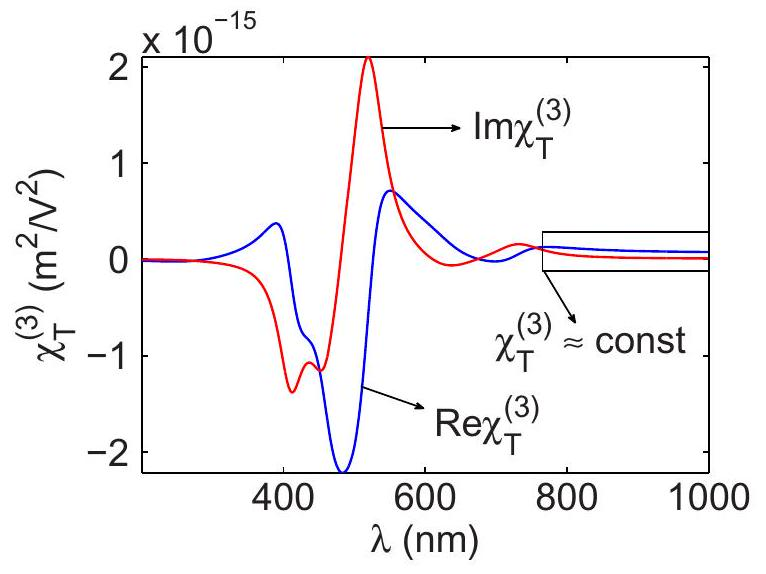
\includegraphics[alt={},max width=\textwidth]{fedff7ea-fb9d-4a80-ac6f-348dbc7a5487-10_574_766_370_500}
\captionsetup{labelformat=empty}
\caption{Figure 3. Thermo-modulational interband nonlinear susceptibility $\chi_{\mathrm{T}}^{(3)}$ as a function of the optical wavelength $\lambda$. Blue and red curves correspond to the real and imaginary parts of $\chi_{\mathrm{T}}^{(3)}(\lambda)$. The region within which $\chi_{\mathrm{T}}^{(3)}$ can be approximately considered to be constant is also indicated.}
\end{center}
\end{figure}

the thermo-modulational nonlinear susceptibility can be approximated as $\chi_{\mathrm{T}}^{(3)} \approx$ const. For ultrashort optical pulses, the calculation of the nonlinear dielectric polarization is more involved.

In the slowly varying envelope approximation (SVEA) the electric field can be expressed as $\vec{E}(t)=\psi(t) \mathrm{e}^{-\mathrm{i} \omega_{0} t} \hat{n}$, where $\omega_{0}$ is the carrier angular frequency, $\hat{n}$ is the polarization unit vector and $\psi(t)$ is the envelope amplitude, which is slowly varying compared to the fast oscillations $\mathrm{e}^{-\mathrm{i} \omega_{0} t}$. The expression for the mean absorbed power per unit volume $P_{\mathrm{A}}(t)$ in this non-monochromatic case includes also the contributions of first-order dispersion and is explicitly given by\\
$P_{\mathrm{A}}(t)=\frac{\epsilon_{0}}{4}\left\{2 \omega_{0} \epsilon_{m}^{\prime \prime}\left(\omega_{0}\right)|\psi|^{2}+\left.\frac{\mathrm{d}\left(\omega \epsilon_{m}^{\prime}\right)}{\mathrm{d} \omega}\right|_{\omega_{0}} \partial_{t}|\psi|^{2}+\left.\mathrm{i} \frac{\mathrm{d}\left(\omega \epsilon_{m}^{\prime \prime}\right)}{\mathrm{d} \omega}\right|_{\omega_{0}}\left(\psi^{*} \partial_{t} \psi-\psi \partial_{t} \psi^{*}\right)\right\}$.

Note that, in the limiting case of infinite pulse duration ( $\psi(t)=\psi_{0}$ ), the expression for $P_{\mathrm{A}}$ converges to the CW result, which is the first term in the expression above $\left(\alpha \epsilon_{m}^{\prime \prime}\left(\omega_{0}\right)|\psi|^{2}\right)$. The second term $\left(\propto \partial_{t}|\psi|^{2}\right)$ does not contribute to the total density of energy absorbed $U_{\mathrm{A}}= \int_{-\infty}^{+\infty} P_{\mathrm{A}}(t) \mathrm{d} t$, since $|\psi|^{2} \rightarrow 0$ for $t \rightarrow \pm \infty$. The last term $\left(\propto \mathrm{i}\left(\psi^{*} \partial_{t} \psi-\psi \partial_{t} \psi^{*}\right)\right)$ depends on the spectral momentum and basically represents the dispersive correction of the first term. In other words, it accounts for the modification of the absorbed power per unit volume $P_{\mathrm{A}}$ within the frequency spectrum of the pulse. In conclusion, the nonlinear polarization created by an ultrafast optical pulse can be expressed in terms of a double convolution integral


\begin{equation*}
\vec{P}_{\mathrm{NL}}(t)=\epsilon_{0} \int_{0}^{+\infty} \mathrm{d} t^{\prime} \int_{0}^{+\infty} \mathrm{d} t^{\prime \prime} \gamma_{\mathrm{T}}\left(t^{\prime}\right) h_{\mathrm{T}}\left(t^{\prime \prime}\right) P_{\mathrm{A}}\left(t-t^{\prime}-t^{\prime \prime}\right) \vec{E}\left(t-t^{\prime}\right) \tag{12}
\end{equation*}


In this expression, $h_{\mathrm{T}}(t)$ is the temporal response function of the TTM and $\gamma_{\mathrm{T}}(t)$ is the interband response function (measured in the units of $\mathrm{m}^{3} \mathrm{~W}^{-1} \mathrm{~s}^{-1}$ ), which is given by the inverse Fourier transform of $\gamma_{\mathrm{T}}(\omega)$ (measured in the units of $\mathrm{m}^{3} \mathrm{~W}^{-1}$ ).

\begin{figure}[h]
\begin{center}
  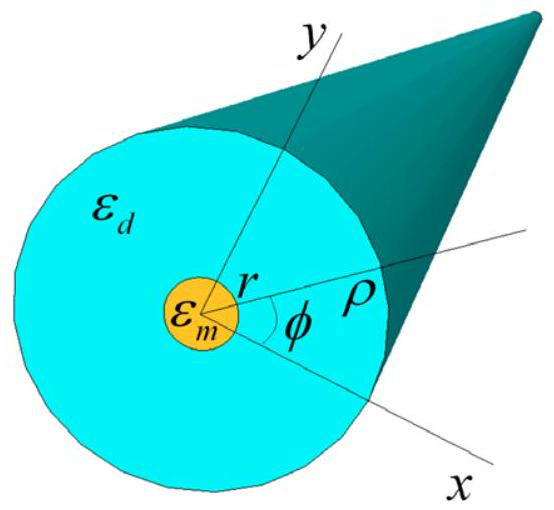
\includegraphics[alt={},max width=\textwidth]{fedff7ea-fb9d-4a80-ac6f-348dbc7a5487-11_510_554_370_502}
\captionsetup{labelformat=empty}
\caption{Figure 4. A gold nanowire of radius $r$ surrounded by silica glass.}
\end{center}
\end{figure}

\section*{5. Thermo-modulational nonlinear dynamics in plasmonic devices}
In the previous sections we have calculated the thermo-modulational interband nonlinear susceptibility of gold starting from the basic properties of its band structure. In this section we study the optical propagation of SPPs guided along gold nanowires surrounded by silica glass, including the novel nonlinear effects originating from the heating of gold. A common theoretical approach to modeling optical propagation in optical fibers and plasmonic waveguides uses the nonlinear Schrödinger equation for the slowly varying amplitude of a guided pulse, perturbatively derived on the assumptions of low loss and nonlinearity [35, 36]. We start the analysis from the time-dependent Maxwell equations for the optical electric ( $\vec{E}$ ) and magnetic ( $\vec{H}$ ) fields, coupled with the nonlinear polarization $\vec{P}_{\mathrm{NL}}(\vec{r}, t)$. As a consequence of the cylindrical symmetry of the gold nanowire around the $z$-axis, the dielectric profile depends solely on the modulus of the position vector $\rho=|\vec{r}|: \epsilon_{L}(\rho, \omega)=\epsilon_{m}(\omega) \theta(r-\rho) +\epsilon_{d}(\omega) \theta(\rho-r)$, where $\theta(x)$ is the Heaviside step function, $\omega$ is the angular frequency, $r$ is the radius of the nanowire and $\epsilon_{m}(\omega), \epsilon_{d}(\omega)$ are the linear dielectric constants of gold and silica. In the calculations below we use the Sellmeier expansion for the dielectric constant of silica $\epsilon_{d}(\omega)$ and a Lorentzian fit to the experimental data [33] for the linear dielectric constant of gold $\epsilon_{m}(\omega)$. A sketch of the plasmonic structure discussed in this section is depicted in figure 4.

\subsection*{5.1. Linear modes}
If one neglects the nonlinear polarization $\vec{P}_{\mathrm{NL}}$, the time-dependent Maxwell equations can be directly solved using the ansatz:


\begin{align*}
& \vec{E}(\vec{r}, t)=I^{1 / 2} \psi \vec{e}(\rho) \mathrm{e}^{\mathrm{i} m \phi+\mathrm{i} \beta z-\mathrm{i} \omega t},  \tag{13}\\
& \vec{H}(\vec{r}, t)=\epsilon_{0} c I^{1 / 2} \psi \vec{h}(\rho) \mathrm{e}^{\mathrm{i} m \phi+\mathrm{i} \beta z-\mathrm{i} \omega t}, \tag{14}
\end{align*}


where $c$ is the speed of light in vacuum, $\psi$ is the mode amplitude (measured in $\mathrm{W}^{1 / 2}$ ), $\vec{e}, \vec{h}$ are the linear guided mode profiles (dimensionless), $\beta$ is the mode propagation constant, $\phi$ is the angle between the vectors $\vec{r}, \hat{x}$ and $m$ is the azimuthal mode order. The factor $I^{1 / 2}$ is a constant, chosen in such a way that $|\psi|^{2}$ represents the total optical power carried by a linear mode with angular frequency $\omega$ and propagation constant $\beta$.

\begin{figure}[h]
\begin{center}
  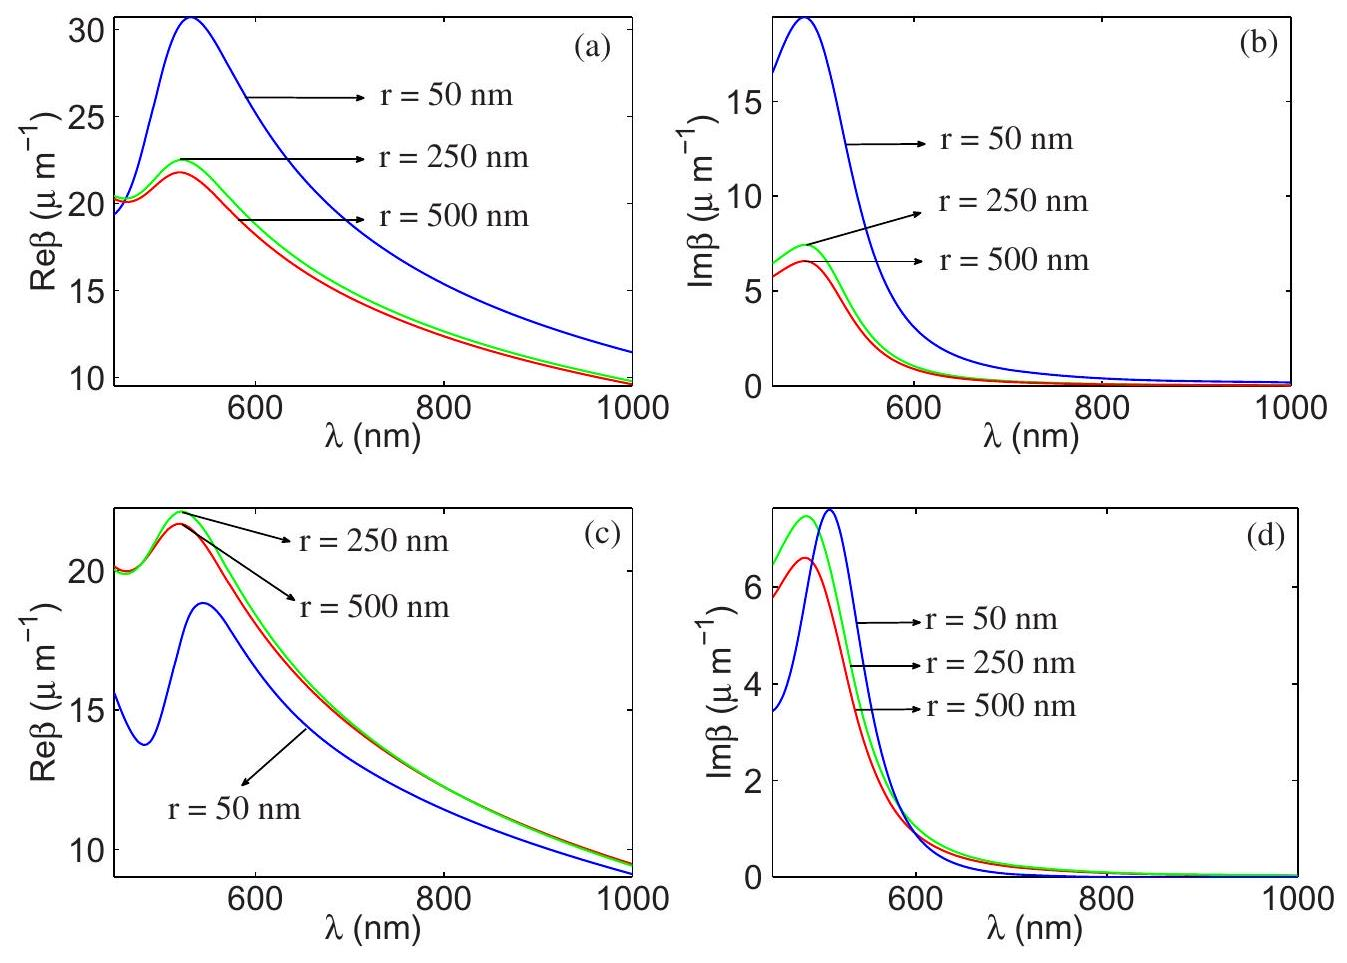
\includegraphics[alt={},max width=\textwidth]{fedff7ea-fb9d-4a80-ac6f-348dbc7a5487-12_963_1347_365_497}
\captionsetup{labelformat=empty}
\caption{Figure 5. Linear dispersion relations (a, c) $\operatorname{Re} \beta(\lambda)$ and (b,d) $\operatorname{Im} \beta(\lambda)$ for the $(\mathrm{a}, \mathrm{b}) m=0$ and $(\mathrm{c}, \mathrm{d}) m=1$ plasmon polariton modes. Blue, green and red curves correspond to the wire radii $r=50,250$ and 500 nm , respectively.}
\end{center}
\end{figure}

The linear dispersion relation $\beta(\omega)$ can be directly calculated by substituting (13) and (14) into the Maxwell equations and by applying the boundary conditions for the continuity of the tangential components of the electric field and the normal component of the displacement vector. The modal profiles $\vec{e}, \vec{h}$ are combinations of modified Bessel and Hankel functions of different orders [36, 37], the solutions $\vec{E}(\vec{r}, t), \vec{H}(\vec{r}, t)$ corresponding to SPPs. Figures $5(\mathrm{a})-(\mathrm{d})$ show the complex dispersion relations (a, c) $\operatorname{Re} \beta(\lambda)$ and $(\mathrm{b}, \mathrm{d}) \operatorname{Im} \beta(\lambda)$ for the $(\mathrm{a}, \mathrm{b}) m=0$ and (c, d) $m=1$ guided SPP modes; the real and imaginary parts of the propagation constant $\beta$ are plotted as functions of the optical wavelength $\lambda$. For both the $m=0,1$ modes, if $\lambda \gtrsim 500 \mathrm{~nm}$, the real ( $\operatorname{Re} \beta$ ) and imaginary ( $\operatorname{Im} \beta$ ) parts of the propagation constant increase as the optical wavelength $\lambda$ decreases, reaching maxima at $\lambda=\lambda_{\mathrm{sp}} \simeq 500 \mathrm{~nm}$, the surface plasmon resonance. For $\lambda \lesssim 500 \mathrm{~nm}$, the behavior of the dispersion relation is more involved. In the ideal case where the metal is lossless, the imaginary part of the propagation constant vanishes, $\operatorname{Im} \beta=0$, whereas the real part $\operatorname{Re} \beta$ diverges as $\lambda \rightarrow \lambda_{\text {sp }}$. Optical confinement depends mainly on the real part of the propagation constant $\operatorname{Re} \beta$ : high values of $\operatorname{Re} \beta$ correspond to tightly confined modes. On the other hand, the attenuation coefficient of the linear modes is directly related to the imaginary part of the propagation constant: $\alpha=2 \operatorname{Im} \beta$. Hence, if one wants to achieve tight SPP confinement it is impossible to avoid high losses so that the use of materials with large gain is required in practical applications [12]. Note that the fundamental mode $m=0$ is TM polarized and that both the real and imaginary parts of the propagation constant $\operatorname{Re} \beta, \operatorname{Im} \beta$ increase as the radius of the gold nanowire decreases (see figures 5(a) and (b)). A contour plot of the time-averaged Poynting vector $S_{z}=(1 / 2) \hat{z} \cdot \operatorname{Re}\left(\vec{E} \times \vec{H}^{*}\right)$ of the TM plasmonic mode

\begin{figure}[h]
\begin{center}
  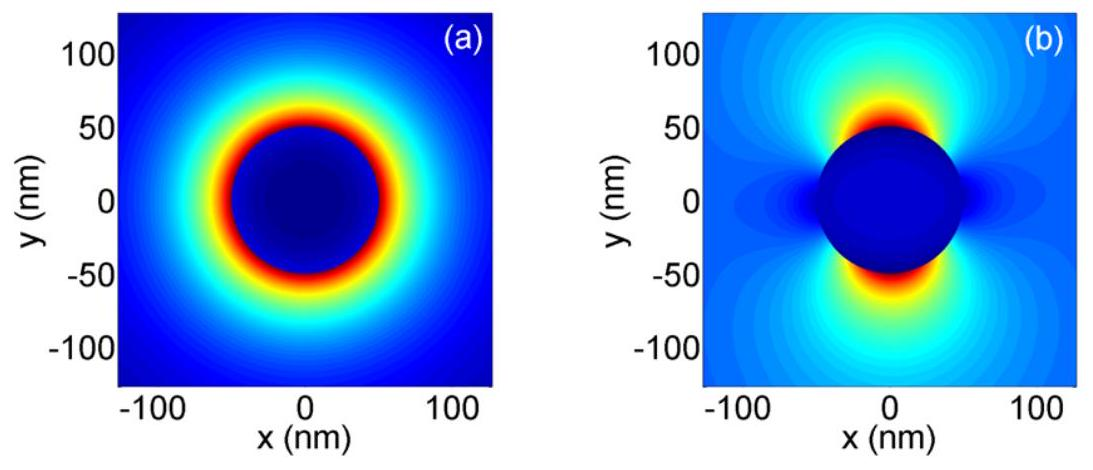
\includegraphics[alt={},max width=\textwidth]{fedff7ea-fb9d-4a80-ac6f-348dbc7a5487-13_470_1093_367_500}
\captionsetup{labelformat=empty}
\caption{Figure 6. Contour plots of the time-averaged Poynting vector for the (a) $m=0$ mode and (b) a superposition of the $m= \pm 1$ modes on a gold nanowire with radius $r=50 \mathrm{~nm}$ surrounded by silica. The optical wavelength is $\lambda=800 \mathrm{~nm}$.}
\end{center}
\end{figure}

\begin{figure}[h]
\begin{center}
  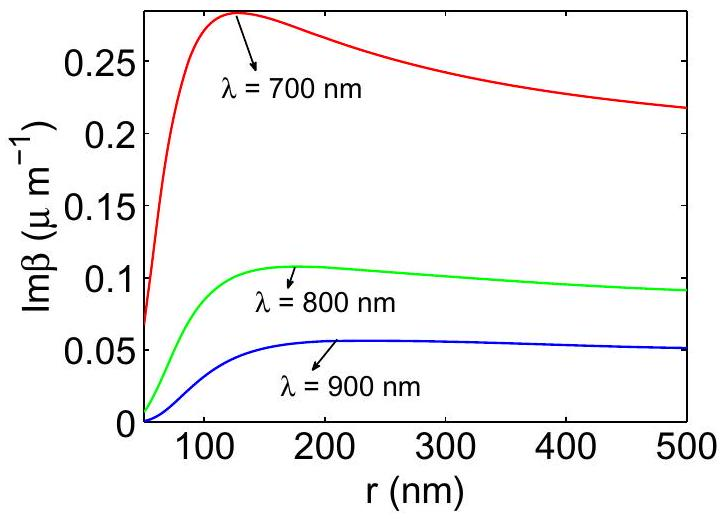
\includegraphics[alt={},max width=\textwidth]{fedff7ea-fb9d-4a80-ac6f-348dbc7a5487-13_519_725_1078_507}
\captionsetup{labelformat=empty}
\caption{Figure 7. Imaginary part of the propagation constant $\operatorname{Im} \beta$ as a function of the wire radius $r$ for the hybrid $m=1$ plasmonic mode. Red, green and blue curves correspond to the optical wavelengths $\lambda=700,800$ and 900 nm , respectively.}
\end{center}
\end{figure}

( $m=0$ ) of a gold nanowire with radius $r=50 \mathrm{~nm}$ at optical wavelength $\lambda=800 \mathrm{~nm}$ is depicted in figure 6(a). Note that the electromagnetic field is tightly bound to the metal surface and that the power distribution is cylindrically symmetric.

In contrast to the TM fundamental mode, the $m=1$ mode is hybrid polarized and less well confined. The dispersion relation does not depend on the sign of the azimuthal mode order $m$ so that the $m= \pm 1$ modes (characterized by opposite chirality) are degenerate. A contour plot of the time-averaged Poynting vector $S_{z}$ of the superposition of $m= \pm 1$ guided SPP modes is shown in figure 6(b) (for the same parameters of figure 6(a)). Note that the power distribution of such a mode is not azimuthally symmetric and depends on the angle $\phi$. If one calculates the time-dependent Poynting vector of the $m= \pm 1$ modes, one finds that these SPPs spiral around the surface of the gold nanowire with opposite chirality [37]. However, the azimuthal spiralling is averaged out in time and as a result there is no net angular flow of time-averaged power for the single $m= \pm 1$ modes and for their superposition. In figure 7 , $\operatorname{Im} \beta$ for the $m=1$ mode is plotted as a function of $r$. Red, green and blue curves correspond to $\lambda=700,800$ and 900 nm , respectively. Both $\operatorname{Re} \beta$ and $\operatorname{Im} \beta$ depend on $r$ in a manner more complicated than for\\
the fundamental TM mode (see figures 5 and 7). In particular, for fixed optical wavelength $\lambda$, $\operatorname{Im} \beta$ is maximum at a characteristic wire radius $r_{0}$, decreasing significantly when $r<r_{0}$. Hence, if the wire radius is much smaller than the optical wavelength $r \ll \lambda$, long-range SPPs can be excited [37]. The field penetration within the gold nanowire is limited for these modes, and hence the attenuation is significantly reduced. In the following nonlinear analysis, we focus on the $m=0,1$ modes. Higher order modes are less well confined and cut off for wavelengths greater than a particular value $\lambda_{\mathrm{co}}$.

\subsection*{5.2. The generalized nonlinear Schrödinger equation}
If the effect of loss and nonlinearity on the fast linear oscillations is weak, the nonlinear propagation of an optical pulse in a plasmonic waveguide can be described by the generalized nonlinear Schrödinger equation (GNLSE) for the field amplitude in the SVEA [35, 36]. In this approach the ansatz for the electromagnetic field is


\begin{align*}
& \vec{E}(\vec{r}, t)=I^{1 / 2} \psi(z, t) \vec{e}(\rho) \mathrm{e}^{\mathrm{i} m \phi+\mathrm{i} \beta_{0} z-\mathrm{i} \omega_{0} t}+\delta \vec{E} \mathrm{e}^{\mathrm{i} m \phi+\mathrm{i} \beta_{0} z-\mathrm{i} \omega_{0} t}  \tag{15}\\
& \vec{H}(\vec{r}, t)=\epsilon_{0} c I^{1 / 2} \psi(z, t) \vec{h}(\rho) \mathrm{e}^{\mathrm{i} m \phi+\mathrm{i} \beta_{0} z-\mathrm{i} \omega_{0} t}+\delta \vec{H} \mathrm{e}^{\mathrm{i} m \phi+\mathrm{i} \beta_{0} z-\mathrm{i} \omega_{0} t} \tag{16}
\end{align*}


where $\psi(z, t)$ is the slowly varying envelope amplitude, $\omega_{0}$ is the carrier angular frequency and $\delta \vec{E}, \delta \vec{H}$ are the residual field corrections due to loss and nonlinearity. We denote $\beta_{0}$ by the linear propagation constant at the carrier frequency calculated by neglecting the nonlinear polarization and the metal loss; $\vec{e}(\rho), \vec{h}(\rho)$ are the corresponding unperturbed linear mode profiles (dimensionless) and $I$ is a constant chosen so that $|\psi|^{2}$ represents the optical power, as in the previous section. For a gold nanowire surrounded by silica glass, the nonlinear polarization is $\vec{P}_{\mathrm{NL}}(\vec{E})=\vec{P}_{\mathrm{NL}}^{\mathrm{Au}}(\vec{E}) \theta(r-\rho)+\vec{P}_{\mathrm{NL}}^{\mathrm{Si}}(\vec{E}) \theta(\rho-r)$, where $\vec{P}_{\mathrm{NL}}^{\mathrm{Si}}(\vec{E})= \left(\epsilon_{0} / 2\right) \chi_{\mathrm{Si}}^{(3)}\left[|\vec{E}|^{2} \vec{E}+(1 / 2) \vec{E}^{2} \vec{E}^{*}\right], \chi_{\mathrm{Si}}^{(3)}=2.25 \times 10^{-22} \mathrm{~m}^{2} \mathrm{~V}^{-2}$ is the Kerr coefficient of silica glass at $\lambda_{0}=800 \mathrm{~nm}$ and $\vec{P}_{\mathrm{NL}}^{\mathrm{Au}}(\vec{E})$ is given by (12). Note that in the expression for the nonlinear polarization of silica glass, we have neglected the Raman effect [38], which should, in principle, be retained. However, as we will show, the effective nonlinear coefficient of silica is much smaller than the effective nonlinear coefficient of gold so that neither Kerr nor Raman effects play any significant role. Hence, for the sake of simplicity, we do not consider the Raman term, comparing our results only with the Kerr term. Since we are mainly interested in the thermo-modulational interband nonlinearity, we neglect the dispersive terms in the absorbed power per unit volume $P_{\mathrm{A}}(t)$, given by (11). These terms are expected to play only a minor role, since they are small corrections to the carrier term. In what follows, we will focus on the spectral region ( $\lambda \approx 800 \mathrm{~nm}$ ) where the interband response function is approximately constant $\left(\gamma_{\mathrm{T}}(\underset{\rightarrow}{\omega}) \approx \gamma_{\mathrm{T}}\left(\omega_{0}\right)\right.$, see figure 3) so that the nonlinear polarization of gold can be approximated by $\vec{P}_{\mathrm{NL}}^{\mathrm{Au}}(\vec{E}) \approx \epsilon_{0} \chi_{\mathrm{Au}}^{(3)}\left(\omega_{0}\right) \int_{0}^{+\infty} \mathrm{d} t^{\prime} h_{\mathrm{T}}\left(t^{\prime}\right)\left|\vec{E}\left(t-t^{\prime}\right)\right|^{2} \vec{E}(t)$. By inserting (15) and (16) into the Maxwell equations, developing a first-order perturbative theory and imposing the Fredholm alternative condition on the residual field corrections $\delta \vec{E}, \delta \vec{H}$ [36], one obtains the GNLSE for the slowly varying amplitude $\psi(z, t)$ :


\begin{equation*}
\mathrm{i} \partial_{z} \psi(z, t)+\hat{D}\left(\mathrm{i} \partial_{t}\right) \psi(z, t)+\Upsilon_{\mathrm{Si}}|\psi(z, t)|^{2} \psi(z, t)+\Upsilon_{\mathrm{Au}} \int_{0}^{+\infty} \mathrm{d} t^{\prime} h_{\mathrm{T}}\left(t^{\prime}\right)\left|\psi\left(z, t-t^{\prime}\right)\right|^{2} \psi(z, t)=0 \tag{17}
\end{equation*}


\begin{figure}[h]
\begin{center}
  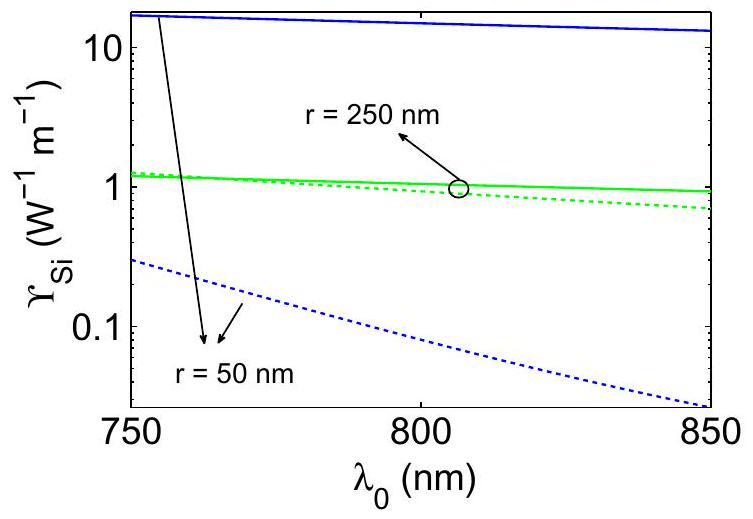
\includegraphics[alt={},max width=\textwidth]{fedff7ea-fb9d-4a80-ac6f-348dbc7a5487-15_519_753_370_502}
\captionsetup{labelformat=empty}
\caption{Figure 8. Kerr nonlinear coefficient ( $\Upsilon_{\mathrm{Si}}$ ) of a gold nanowire surrounded by silica glass for the $m=0$ (full lines) and $m=1$ (dashed lines) modes. Blue and green lines correspond to the wire radii $r=50$ and 250 nm , respectively. Note that the plot is made in the semi-logarithmic scale.}
\end{center}
\end{figure}

where

$$
\begin{aligned}
& \Upsilon_{\mathrm{Si}}=\frac{\omega_{0} \chi_{\mathrm{Si}}^{(3)}}{4 \epsilon_{0} c^{2}} \frac{\int_{0}^{2 \pi} \mathrm{~d} \phi \int_{r}^{+\infty} \mathrm{d} \rho \rho\left[2|\vec{e}|^{4}+\left|\vec{e}^{2}\right|^{2}\right]}{\left(\int_{0}^{2 \pi} \mathrm{~d} \phi \int_{0}^{+\infty} \mathrm{d} \rho \rho \operatorname{Re}\left[\vec{e} \times \vec{h}^{*}\right] \cdot \hat{z}\right)^{2}} \\
& \Upsilon_{\mathrm{Au}}=\frac{\omega_{0} \chi_{\mathrm{Au}}^{(3)}}{\epsilon_{0} c^{2}} \frac{\int_{0}^{2 \pi} \mathrm{~d} \phi \int_{0}^{r} \mathrm{~d} \rho \rho|\vec{e}|^{4}}{\left(\int_{0}^{2 \pi} \mathrm{~d} \phi \int_{0}^{+\infty} \mathrm{d} \rho \rho \operatorname{Re}\left[\vec{e} \times \vec{h}^{*}\right] \cdot \hat{z}\right)^{2}}
\end{aligned}
$$

The linear dispersion operator $\hat{D}\left(\mathrm{i} \partial_{t}\right)$ is complex, accounting as it does for the linear losses of gold. Its action on the envelope amplitude can be calculated in the Fourier domain:


\begin{equation*}
\hat{D}\left(\mathrm{i} \partial_{t}\right) \psi(z, t)=\frac{1}{2 \pi} \int_{-\infty}^{+\infty} \mathrm{d} \Delta \omega D_{\omega_{0}}(\Delta \omega) \psi(z, \Delta \omega) \mathrm{e}^{-\mathrm{i} \Delta \omega t} \tag{18}
\end{equation*}


where $\Delta \omega=\omega-\omega_{0}$ and $D_{\omega_{0}}(\Delta \omega)=\beta\left(\omega_{0}+\Delta \omega\right)-\beta_{0}-\left.\frac{\mathrm{d} \beta^{\prime}}{\mathrm{d} \omega}\right|_{\omega_{0}} \Delta \omega$. Note that $\beta_{0}$ is the realvalued carrier propagation constant of the linear unperturbed mode, $\beta(\omega)$ is the complex modal wavevector calculated in the previous section and the prime in the equation above indicates the real part ( $\beta^{\prime}=\operatorname{Re} \beta$ ). The nonlinear parameters $\Upsilon_{\mathrm{Si}}, \Upsilon_{\mathrm{Au}}$ are measured in $\mathrm{m}^{-1} \mathrm{~W}^{-1}$ and account also for the surface nonlinearity [36]. Note that while $\Upsilon_{\mathrm{Si}}$ is a real quantity, $\Upsilon_{\mathrm{Au}}$ is complex and accounts for the nonlinear loss of gold. The nonlinear parameters of silica ( $\Upsilon_{\mathrm{Si}}$ ) and gold ( $\Upsilon_{\mathrm{Au}}$ ) are plotted as functions of the carrier wavelength $\lambda_{0}$ in figures 8, 9(a) and (b). In both figures, the full and dashed curves represent the $m=0$ and 1 modes, while blue and green colors correspond to wire radii $r=50$ and 250 nm . Note that the real part of the gold nonlinear parameter is much greater than the Kerr nonlinear parameter of silica in the spectral region considered. Also, if $r \ll \lambda$, the nonlinear parameters of the $m=1$ mode are much smaller than those for the $m=0$ mode since they are much less confined. In this limit, as discussed in the previous section, while the fundamental $m=0$ mode is tightly confined to the metal surface and propagates only for a few wavelengths, the $m=1$ mode is much less localized and can

\begin{figure}[h]
\begin{center}
  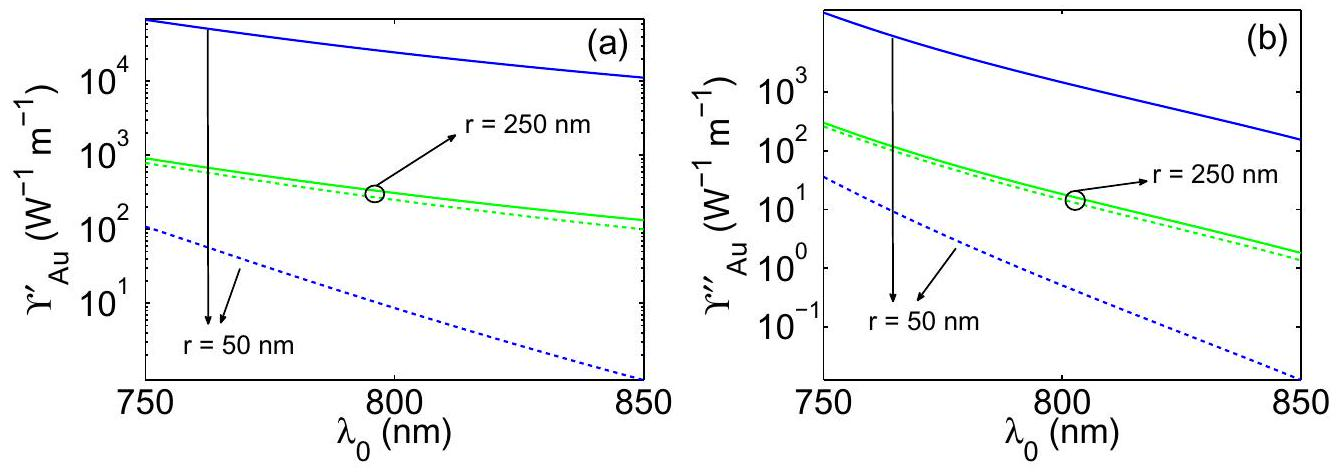
\includegraphics[alt={},max width=\textwidth]{fedff7ea-fb9d-4a80-ac6f-348dbc7a5487-16_474_1342_372_502}
\captionsetup{labelformat=empty}
\caption{Figure 9. (a) The real and (b) imaginary parts of the thermo-modulational interband nonlinear coefficient ( $\Upsilon_{\mathrm{Au}}$ ) of a gold nanowire surrounded by silica glass for $m=0$ (full curves) and $m=1$ (dashed curves) modes. Blue and green curves correspond to the wire radii $r=50$ and 250 nm , respectively. Note that the plots are made in the semi-logarithmic scale.}
\end{center}
\end{figure}

\begin{figure}[h]
\begin{center}
  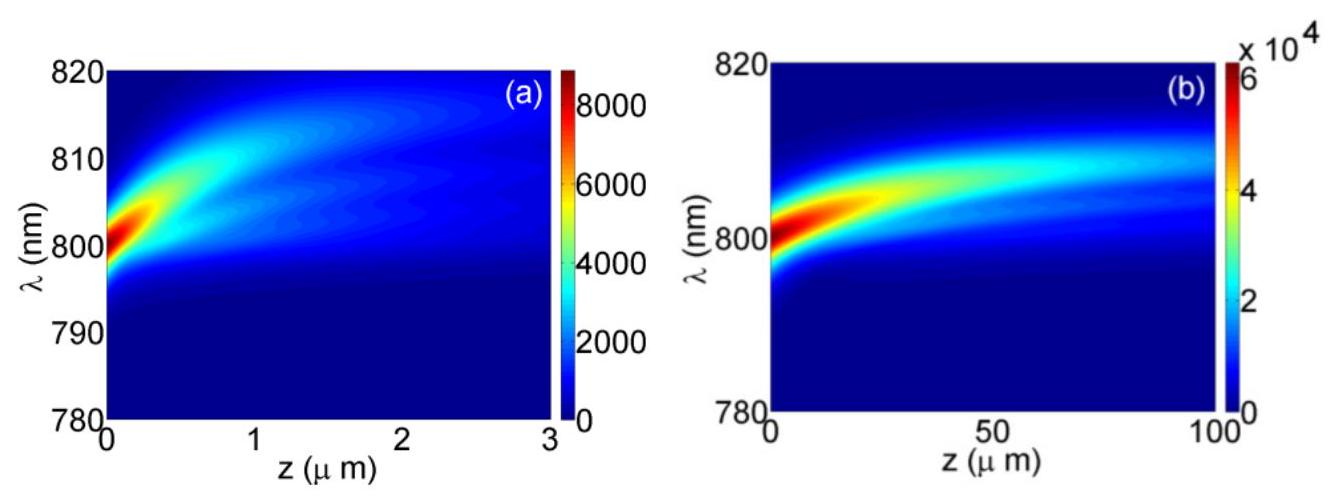
\includegraphics[alt={},max width=\textwidth]{fedff7ea-fb9d-4a80-ac6f-348dbc7a5487-16_499_1340_1158_495}
\captionsetup{labelformat=empty}
\caption{Figure 10. Nonlinear propagation of an optical pulse along a gold nanowire with radius $r=50 \mathrm{~nm}$ surrounded by silica glass for: (a) $m=0$ and an instantaneous input power $P_{\text {in }}=1 \times 10^{4} \mathrm{~W}$; (b) $m=1$ and an instantaneous input power $P_{\text {in }}= 5.3 \times 10^{5} \mathrm{~W}$. In both figures the input pulse is a hyperbolic secant $\psi(0, t)= \sqrt{P_{\text {in }}} \operatorname{sech}\left(t / t_{0}\right)$, with $t_{0}=106 \mathrm{fs}$. The contour plot displays the modulus of the Fourier transform of the optical amplitude: $|\psi(z, \omega)|$.}
\end{center}
\end{figure}

propagate for longer distances (long-range guided SPP mode). This reduction in loss is at the cost of a weaker effective nonlinearity.

The formulation of the propagation equation (17) constitutes the main result of this paper. We have numerically solved (17) using the fast Fourier split-step algorithm. As we have already shown, when $\lambda_{0} \approx 800 \mathrm{~nm}$ the Kerr nonlinearity of silica does not play a significant role and can be neglected. For the numerical simulations we have considered a hyperbolic secant input pulse: $\psi(0, t)=\sqrt{P_{\text {in }}} \operatorname{sech}\left(t / t_{0}\right)$, with $t_{0}=106 \mathrm{fs} . P_{\text {in }}$ is the instantaneous pulse power, which can be directly calculated from the average power of the laser source: $P_{\text {in }}=C_{\text {eff }} P_{\text {av }} /\left(2 v_{\text {rep }} t_{0}\right)$, where $C_{\text {eff }}$ is the launch efficiency of the laser beam into the gold nanowire, $\nu_{\text {rep }}$ is the repetition rate and $2 t_{0}$ is the pulse duration. The instantaneous power is kept well below the damage threshold power of gold, above which melting, ablation and vaporization occur

\begin{figure}[h]
\begin{center}
  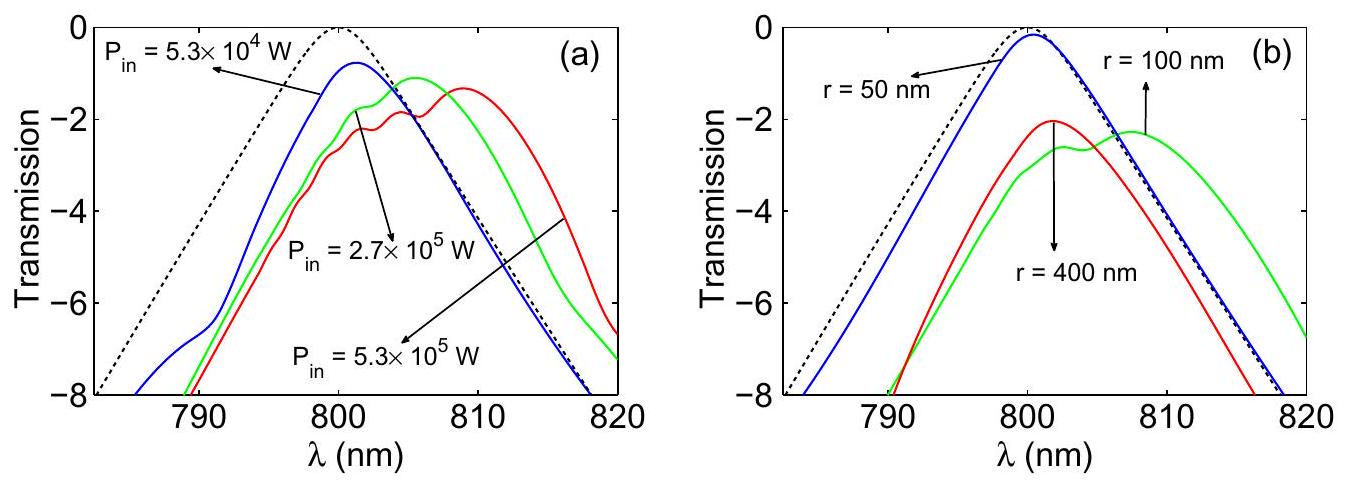
\includegraphics[alt={},max width=\textwidth]{fedff7ea-fb9d-4a80-ac6f-348dbc7a5487-17_488_1347_367_502}
\captionsetup{labelformat=empty}
\caption{Figure 11. Transmission spectrum $\left(\mathcal{T}=\ln \left|\psi(L, \omega) / \psi_{0 M}\right|\right.$, where $\psi_{0 M}= \max [\psi(0, \omega)])$ of the $m=1$ long-range mode. (a) $\mathcal{T}$ is calculated at a propagation length of $L=100 \mu \mathrm{~m}$, for a fixed wire radius of $r=50 \mathrm{~nm}$ and for different input optical powers: $P_{\text {in }}=5.3 \times 10^{4} \mathrm{~W}$ (blue curve), $P_{\text {in }}= 2.7 \times 10^{5} \mathrm{~W}$ (green curve) and $P_{\text {in }}=5.3 \times 10^{5} \mathrm{~W}$ (red curve). (b) Transmission spectrum $(\mathcal{T})$ for a propagation length of $L=20 \mu \mathrm{~m}$, fixed input power $P_{\text {in }}= 5.3 \times 10^{4} \mathrm{~W}$ and for different nanowire radii: $r=50 \mathrm{~nm}$ (blue curve), $r=$ 100 nm (green curve) and $r=400 \mathrm{~nm}$ (red curve). The black dashed curves represent the input spectrum $\left(\ln \left|\psi(0, \omega) / \psi_{0 M}\right|\right)$.}
\end{center}
\end{figure}

( $P_{\text {dam }} \approx 10^{6} \mathrm{~W}$ ) [39]. In figures 10(a) and (b), the numerical propagation along a gold nanowire with radius $r=50 \mathrm{~nm}$ surrounded by silica glass is depicted for (a) $m=0, P_{\text {in }}=1 \times 10^{4} \mathrm{~W}$ and (b) $m=1, P_{\text {in }}=5.3 \times 10^{5} \mathrm{~W}$. In this contour plot the modulus of the Fourier transform of the optical amplitude $(|\psi(z, \omega)|)$ is shown. The $m=0$ TM mode is highly nonlinear and significant nonlinear dynamics can be observed even for relatively small optical power. However, such a high nonlinearity is paid for by high loss, limiting the effective propagation length to $L \approx 2 \mu \mathrm{~m}$ (see figure 10(a)). The hybrid polarized $m=1$ mode supports long-range guided SPP modes so that both the nonlinear and loss coefficients are significantly smaller. In this case, in order to observe a strong nonlinear dynamics, it is necessary to use a considerably higher optical power. For the $m=0,1$ modes a signature red-shift indicates the presence of a thermo-modulational interband nonlinearity, analogously to the Raman effect [38].

This red-shift is the natural consequence of the intrinsic delayed mechanism governing the thermo-modulational interband nonlinear susceptibility of gold. In the time domain the frequency red-shift is accompanied by a small pulse delay of order $\approx 1 \mathrm{fs}$. We emphasize that neither the Kerr nor the Raman nonlinearities of silica are large enough to produce the reported red-shift for the propagation lengths considered. The strong red-shift is accompanied by a large time-delayed nonlinear loss, as can be understood from figures 11(a) and (b). In figure 11(a), the transmission spectrum $\left(\mathcal{T}=\ln \left|\psi(L, \omega) / \psi_{0 M}\right|\right.$, where $\psi_{0 M}=\max [\psi(0, \omega)]$ and $L=100 \mu \mathrm{~m})$ of the $m=1$ long-range mode of a gold nanowire with radius $r=50 \mathrm{~nm}$ is depicted for several input powers: $P_{\text {in }}=5.3 \times 10^{4} \mathrm{~W}$ (blue curve), $P_{\text {in }}=2.7 \times 10^{5} \mathrm{~W}$ (green curve) and $P_{\text {in }}=5.3 \times 10^{5} \mathrm{~W}$ (red curve). The black dashed curve corresponds to the normalized input spectrum on a logarithmic scale $\left(\ln \left|\psi(0, \omega) / \psi_{0 M}\right|\right)$. Note that as the input power increases the red-shift increases and the transmission peak decreases accordingly as a consequence of nonlinear loss. Also, as the power increases, the transmission spectrum displays some weak oscillations, which resemble Kerr-related self-phase modulation. Indeed, the dispersion length is

\begin{figure}[h]
\begin{center}
  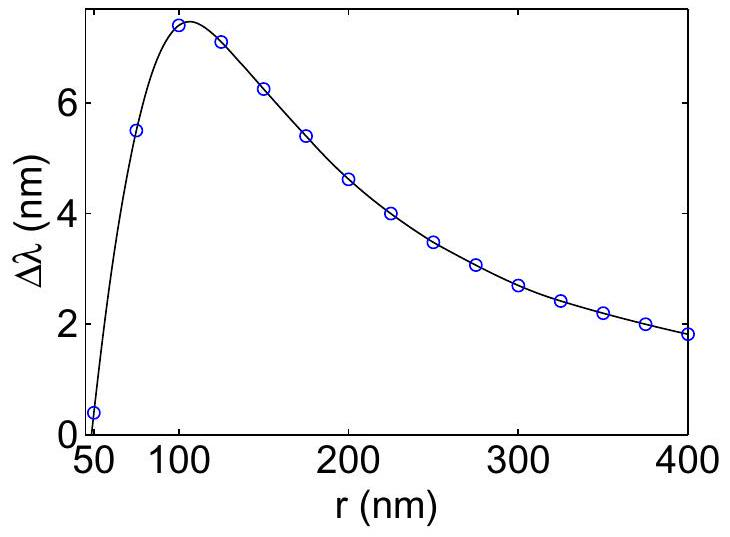
\includegraphics[alt={},max width=\textwidth]{fedff7ea-fb9d-4a80-ac6f-348dbc7a5487-18_537_730_370_504}
\captionsetup{labelformat=empty}
\caption{Figure 12. The wavelength red-shift $\Delta \lambda$ as a function of the wire radius $r$ for the $m=1$ long-range mode, a fixed input power $P_{\text {in }}=5.3 \times 10^{4} \mathrm{~W}$ and the propagation length $L=20 \mu \mathrm{~m}$. Blue circles are the results of numerical simulations, while the full black curve is an interpolation of the numerical results.}
\end{center}
\end{figure}

much longer than the nonlinear length so that only the linear loss affects the nonlinear dynamics. In figure 11(b), the transmission spectrum $\left(\mathcal{T}=\ln \left|\psi(L, \omega) / \psi_{0 M}\right|\right.$, where $\left.L=20 \mu \mathrm{~m}\right)$ of the $m=1$ long-range mode is shown for several nanowire radii: $r=50 \mathrm{~nm}$ (blue curve), $r=100 \mathrm{~nm}$ (green curve) and $r=400 \mathrm{~nm}$ (red curve). The black dashed curve represents the input spectrum $\left(\ln \left|\psi(0, \omega) / \psi_{0 M}\right|\right)$ and the input power is fixed at $P_{\text {in }}=5.3 \times 10^{4} \mathrm{~W}$. Note that the linear properties of the $m=1$ mode are non-trivial (see figure 7) and, as a consequence, the power dependence of the red-shift and the transmission peak is non-monotonic. This means that an optimal radius $r=r_{\mathrm{o}}$ exists, where the achievable red-shift is maximum. In figure 12, the redshift of the transmission peak of the $m=1$ long-range mode is plotted as a function of wire radius for a fixed input power $P_{\text {in }}=5.3 \times 10^{4} \mathrm{~W}$ and for a propagation distance $L=20 \mu \mathrm{~m}$. The open blue circles represent the results of numerical simulations, whereas the black curve corresponds to an interpolation of the numerical results. The maximum red-shift attainable at this input power is $\Delta \lambda \approx 7 \mathrm{~nm}$ for a radius of $r_{\mathrm{o}} \approx 110 \mathrm{~nm}$. The dependence of the thermomodulational interband nonlinear coefficient ( $\Upsilon_{\mathrm{Au}}$ ) and the absorption coefficient ( $\alpha=2 \beta_{0}^{\prime \prime}$ ) on $r$ strongly affects the nonlinear dynamics and as a consequence the red-shift attainable, which reaches a maximum at $r=r_{\mathrm{o}}$. When the input power increases, the maximum red-shift increases accordingly.

\section*{6. Summary}
In this paper we have described the thermo-modulational interband nonlinearity of gold starting from its band structure. Electrons in the conduction band are heated by an ultrashort optical pulse and the interband dielectric properties are modulated accordingly. Using a semiclassical approach, we have calculated the imaginary part of the dielectric constant of gold, accounting for interband absorption, which basically depends on the JDOS. In turn, we have been able to describe the temperature dependence of the dielectric susceptibility of gold and have modeled the heating and the relaxation of the conduction electrons using a TTM. We discovered that the metal nonlinearity is basically characterized by a delayed mechanism, similar to the Raman\\
effect in some senses, but with a much longer response time ( $\approx 300 \mathrm{fs}$ ). Also, in contrast to the Raman effect, the thermo-modulational interband susceptibility is complex valued, providing a delayed nonlinear loss or gain. The optical propagation of SPPs is strongly affected by the metal nonlinearity, which we have found to be several orders of magnitude larger than the Kerr nonlinearity of fused silica. We have derived, for the first time to our knowledge, a GNLSE suitable for modeling the optical propagation of SPPs along a gold nanowire surrounded by silica glass. Solving this equation using a fast Fourier split step algorithm, we found that the signature of the thermo-modulational interband nonlinearity is a red-shift of the optical pulse. This red-shift results from the intrinsic time-delayed nature of the thermo-modulational interband nonlinearity of gold. We believe that this novel nonlinear effect may be important for frequency conversion in plasmonic devices. We have also provided some details of the expected red-shift, its dependence on the wire radius and the optical power necessary to observe it experimentally.

\section*{Acknowledgments}
This research was supported by the German Max Planck Society for the Advancement of Science (MPG). MC acknowledges financial support from the Fondazione Cariplo through the project 'Engineering of optical nonlinearities in plasmonic metamaterials' (grant no. 20100595). GDV and SL acknowledge financial support from the Fondazione Cariplo through the project 'New Frontiers in Plasmonic Nanosensing' (grant no. 2011-0338).

\section*{References}
[1] Veselago V G 1968 Sov. Phys.-Usp. 10509\\[0pt]
[2] Pendry J B 2000 Phys. Rev. Lett. 853966\\[0pt]
[3] Schurig D, Mock J J, Justice B J, Cummer S A, Pendry J B, Starr A F and Smith D R 2006 Science 314977\\[0pt]
[4] Soukoulis C M and Wegener M 2011 Nature Photon. 5523\\[0pt]
[5] Klein M W, Enkrich C, Wegener M and Linden S 2006 Science 313502\\[0pt]
[6] Liu Y, Bartal G, Genov D A and Zhang X 2007 Phys. Rev. Lett. 99153901\\[0pt]
[7] Ciattoni A, Rizza C and Palange E 2011 Phys. Rev. A 83043813\\[0pt]
[8] Schmidt M A, Sempere L N P, Tyagi H K, Poulton C G and Russell P St J 2008 Phys. Rev. B 77033417\\[0pt]
[9] Bozhevolnyi S I, Volkov V S, Devaux E, Laluet J Y and Ebbesen T W 2006 Nature 440508\\[0pt]
[10] Gobin A M, Lee M H, Halas N J, James W D, Drezek R A and West J L 2007 Nano Lett. 71929\\[0pt]
[11] Vedantam S, Lee H, Tang J, Conway J, Staffaroni M and Yablonovitch E 2009 Nano Lett. 93447\\[0pt]
[12] Gather M C, Meerholz K, Danz N and Leosson K 2010 Nature Photon. 4457\\[0pt]
[13] Zayats A V and Richards D 2009 Nano-Optics and Near-Field Optical Microscopy (Boston, MA: Artech House)\\[0pt]
[14] MacDonald K F, Samson Z L, Stockman M I and Zheludev N I 2009 Nature Photon. 355\\[0pt]
[15] Davoyan A R, Shadrivov I V, Zharov A A, Gramotnev D K and Kivshar Y S 2010 Phys. Rev. Lett. 105116804\\[0pt]
[16] Feigenbaum E and Orenstein M 2007 Opt. Lett. 32674\\[0pt]
[17] Marini A and Skryabin D V 2010 Phys. Rev. A 81033850\\[0pt]
[18] Noskov R E, Belov P A and Kivshar Y S 2012 Phys. Rev. Lett. 108093901\\[0pt]
[19] Noskov R E, Krasnok A E and Kivshar Y S 2012 New J. Phys. 14093005\\[0pt]
[20] Dionne J A, Verhagen E, Polman A and Atwater H A 2008 Opt. Express 1619001\\[0pt]
[21] Conforti M, Guasoni M and De Angelis C 2008 Opt. Lett. 332662\\[0pt]
[22] Della Valle G and Longhi S 2010 Opt. Lett. 35673\\[0pt]
[23] Alú A and Engheta N 2009 Phys. Rev. Lett. 102233901\\[0pt]
[24] Lee T K, Bristow A D, Hubner J and van Driel H M 2006 J. Opt. Soc. Am. B 232142\\[0pt]
[25] Rotenberg N, Bristow A D, Pfeiffer M, Betz M and van Driel H M 2007 Phys. Rev. B 75155426\\[0pt]
[26] Davoyan A R 2011 Phys. Lett. A 3751615\\[0pt]
[27] Rosei R and Lynch D W 1972 Phys. Rev. B 53883\\[0pt]
[28] Guerrisi M, Rosei R and Winsemius P 1975 Phys. Rev. B 12557\\[0pt]
[29] Sun C K, Vallée F, Acioli L H, Ippen E P and Fujimoto J G 1994 Phys. Rev. B 5015337\\[0pt]
[30] Baida H, Mongin D, Christofilos D, Bachelier G, Crut A, Maioli P, Del Fatti N and Vallée F 2011 Phys. Rev. Lett. 107057402\\[0pt]
[31] Carpene E 2006 Phys. Rev. B 74024301\\[0pt]
[32] Conforti M and Della Valle G 2012 Phys. Rev. B 85245423\\[0pt]
[33] Johnson P B and Christy R W 1972 Phys. Rev. B 64370\\[0pt]
[34] Suffczynski M 1960 Phys. Rev. 117663\\[0pt]
[35] Afshar S V and Monro T M 2009 Opt. Express 172298\\[0pt]
[36] Marini A, Hartley R, Gorbach A V and Skryabin D V 2011 Phys. Rev. A 84063839\\[0pt]
[37] Schmidt M A and Russell P St J 2008 Opt. Express 1613617\\[0pt]
[38] Blow K J and Wood D 1989 IEEE J. Quantum Electron. 252665\\[0pt]
[39] Stuart B C, Feit M D, Herman S, Rubenchik A M, Shore B W and Perry M D 1996 J. Opt. Soc. Am. B 13459


\end{document}